\documentclass[aspectratio=169]{beamer}
\usepackage{will_handley_beamer}
\usepackage{title_page}
\usepackage{slashed}
\usetikzlibrary{positioning}
\usetikzlibrary{calc}
\usetikzlibrary{fit}
\usepackage[percent]{overpic}

% Commands
% --------
% - \arxiv{arxiv number}
% - \arxiv{<number>}            arxiv.org/abs/<number>
% - \oldarxiv{<arxiv number>}   arxiv.org/<number>
% - \doi{<doi>}                 doi.org/<doi>
% - \xkcd{<number>}             xkcd.com/<number>
% - \email{<email>}             <<email>>
% - \tthref{<website>}          <website>
% - \av[dist]{<quantity>}       <quantity>_{dist}

% Talk details
% ------------
\title{Next-generation statistical inference tools}
\subtitle{Simulation-based inference, marginal statistics \& accelerated nested sampling}
\date{13\textsuperscript{th} November 2024}

\begin{document}
%The most relevant branches are: `remotes/origin/ras_sbi_2024`, `remotes/origin/lcdm_2023`, `remotes/origin/tools_2021`, `remotes/origin/cavendish_2024`, `remotes/origin/cosmoverse_2024`, and `remotes/origin/adelaide_2020`.  Some older branches like `remotes/origin/garching_2015` and `remotes/origin/edinburgh_2016` also have useful introductory material on Nested Sampling, but the figures and explanations may be slightly outdated.
% Also phystat_2024 and phystat_imperial_2024



%- [X] take the sydney talk as base
%  -[ ] borrow some old slides for MCMC-based comparison (particularly relevant for the global fit) 
%-[X] Nested Sampling & MCMC
%-[X] SBI
%  -[X] Take these from sydney talk 
%-[X] Margarine
%  -[X] take these from?? 
%    -[X] oxford? 
%- [ ] Accelerated nested sampling
%- [X] JaxNS
%- [ ] Add CPNest arxiv link to zoo
%- [ ] Add REACH arxiv link

% TODO:
% - reduce emphasis on nested sampling
% - put in slides

\begin{frame}
    \titlepage
\end{frame}

\begin{frame}
    \frametitle{LBI: Likelihood-based inference}
    \begin{columns}
        \column{0.5\textwidth}
        The standard approach if you are fortunate enough to have a likelihood function $\only<1-2>{P(D|\theta)}\only<3->{\C[2]{\mathcal{L}(D|\theta)}}$: 
        \[
            \only<1-2>{
                P(\theta|D) = \frac{P(D|\theta)P(\theta)}{P(D)}
            }
            \only<2>{
                \qquad
                \C[0]{\text{Posterior}} = \frac{\C[2]{\text{Likelihood}}\times\C[1]{\text{Prior}}}{\C[3]{\text{Evidence}}}
            }
            \only<3>{
                \C[0]{\mathcal{P}(\theta|D)} = \frac{\C[2]{\mathcal{L}(D|\theta)}\C[1]{\pi(\theta)}}{\C[3]{\mathcal{Z}(D)}}
                \qquad
                \C[0]{\text{Posterior}} = \frac{\C[2]{\text{Likelihood}}\times\C[1]{\text{Prior}}}{\C[3]{\text{Evidence}}}
            }
            \only<4>{
                \C[0]{P(\theta|D)} \C[3]{P(D)} = \C[4]{P(\theta,D)} = \C[2]{P(D|\theta)}\C[1]{P(\theta)}, \qquad
            }
            \only<5>{
                \C[0]{\mathcal{P}}\times\C[3]{\mathcal{Z}} = \C[4]{\mathcal{J}} = \C[2]{\mathcal{L}}\times\C[1]{\pi}, \qquad \C[4]{\text{Joint}} = \C[4]{\mathcal{J}} = P(\theta,D)
            }
        \]
        \vspace{-10pt}
        \begin{enumerate}
            \item Define \C[1]{prior $\pi(\theta)$} 
                \begin{itemize}
                    \item spend some time being philosophical
                \end{itemize}
            \item Sample \C[0]{posterior $\mathcal{P}(\theta|D)$} 
                \begin{itemize}
                    \item use out-of-the-box MCMC tools such as\\ \texttt{emcee} or \texttt{MultiNest}
                    \item make some triangle plots
                \end{itemize}
            \item Optionally compute \C[3]{evidence $\mathcal{Z}(D)$}
                \begin{itemize}
                    \item e.g. nested sampling or parallel tempering
                    \item do some model comparison (i.e. science)
                    \item talk about tensions
                \end{itemize}
        \end{enumerate}
        \column{0.5\textwidth}
        \hfill%
        \begin{overpic}[width=0.6\textwidth]{figures/des_parameters.pdf}
            \put(-40,90) {DES Y5 SN Ia}
            \put(-40,80) {\arxiv{2401.02929}}
        \end{overpic}
        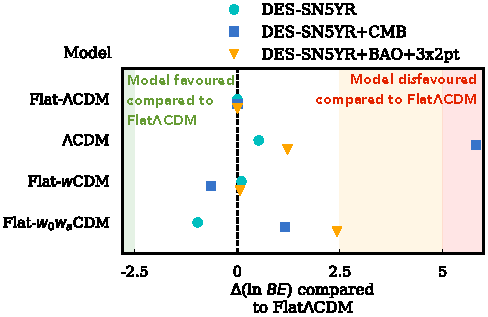
\includegraphics[width=0.5\textwidth]{figures/des_model_comparison.pdf}%
        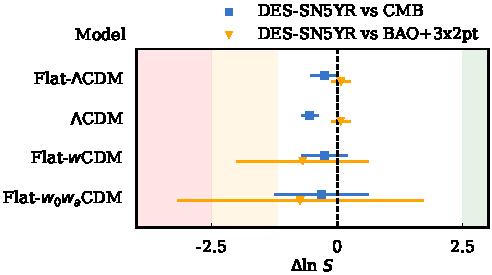
\includegraphics[width=0.5\textwidth]{figures/des_suspiciousness.pdf}
    \end{columns}
\end{frame}

\begin{frame}
    \frametitle{The three pillars of Bayesian inference}
    \begin{columns}[t]
        \column{0.33\textwidth}
        \begin{block}{Parameter estimation}
            What do the data tell us about the parameters of a model?\\
            \only<1>{\textit{e.g. the size or age of a $\Lambda$CDM universe}}%
            \only<2>{\textit{e.g. the masses and spins of a BBH collision}}
            \[ \hspace{-4pt}\C[0]{P(\theta|D,M)} = \frac{\C[2]{P(D|\theta,M)} \C[1]{P(\theta|M)}}{\C[3]{P(D|M)}} \] 
            \[ \C[0]{\mathcal{P}} = \frac{\C[2]{\mathcal{L}} \times\C[1]{\pi}}{\C[3]{\mathcal{Z}}}\] 
            \[ \C[0]{\text{Posterior}} = \frac{\C[2]{\text{Likelihood}} \times\C[1]{\text{Prior}}}{\C[3]{\text{Evidence}}}\]
        \end{block}
        \column{0.3\textwidth}
        \begin{block}{Model comparison}
            How much does the data support a particular model?\\
            \only<1>{\textit{e.g. $\Lambda$CDM vs a dynamic dark energy cosmology}}%
            \only<2>{\textit{e.g. IMRPhenom vs EOBNR waveform models}}
            \[ \C[5]{P(M|D)} = \frac{\C[3]{P(D|M)} \C[6]{P(M)}}{\C[7]{P(D)}} \vspace{-7pt}\]
            \[ \frac{\C[3]{\mathcal{Z}_{M}} \C[6]{\Pi_{M}}}{\C[7]{\sum_m Z_m \Pi_m}} \]
            \[ \C[5]{\text{Posterior}} = \frac{\C[3]{\text{Evidence}} \times\C[6]{\text{Prior}}}{\C[7]{\text{Normalisation}}}\]
        \end{block}
        \column{0.33\textwidth}
        \begin{block}{Tension quantification}
            Do different datasets make consistent predictions from the same model? 
            \only<1>{\textit{\textit{e.g. CMB vs Type IA supernovae data}}}%
            \only<2>{\textit{e.g. Automated glitch detection}}
            \[ \mathcal{R} = \frac{\C[3]{\mathcal{Z}}_{AB}}{\C[3]{\mathcal{Z}}_A\C[3]{\mathcal{Z}}_\mathcal{B}}\] 
            \[
                \begin{aligned} \log\mathcal{S} = \av[{\C[0]{\mathcal{P}}_{AB}}]{\C[2]{\log\mathcal{L}}_{AB}}&\\
                    -\av[{\C[0]{\mathcal{P}}_{A}}]{\C[2]{\log\mathcal{L}}_{A}}&\\
                    -\av[{\C[0]{\mathcal{P}}_{B}}]{\C[2]{\log\mathcal{L}}_{B}}&
                \end{aligned}
            \]
        \end{block}
    \end{columns}
\end{frame}

\begin{frame}
    \frametitle{Model comparison $\C[3]{\mathcal{Z}=P(D|M)}$}
    \begin{itemize}
        \item Bayesian model comparison allows mathematical derivation of key philosophical principles.
    \end{itemize}
    \begin{columns}[t]
        \column{0.47\textwidth}
        Viewed from data-space $D$:
        \begin{block}{Popper's falsificationism}
            \begin{itemize}
                \item Prefer models that make bold predictions.
                \item if proven true, model more likely correct.
            \end{itemize}
        \end{block}
        \includegraphics<1|handout:0>[width=\textwidth, page=1]{figures/popper}%
        \includegraphics<2|handout:0>[width=\textwidth, page=2]{figures/popper}%
        \includegraphics<3>[width=\textwidth, page=3]{figures/popper}%
        \begin{itemize}
            \item Falsificationism comes from normalisation
        \end{itemize}
        \column{0.47\textwidth}
        Viewed from parameter-space $\theta$:
        \begin{block}{Occam's razor}
            \begin{itemize}
                \item Models should be as simple as possible
                \item \ldots but no simpler
            \end{itemize}
        \end{block}
        \begin{itemize}
            \item Occam's razor equation:
                \[\C[3]{\log\mathcal{Z}} = \av[{\C[0]{\mathcal{P}}}]{\C[2]{\log\mathcal{L}}} - \mathcal{D}_\text{KL}\]
            \item ``Occam penalty'': KL divergence between \C[1]{prior~$\pi$} and \C[0]{posterior~$\mathcal{P}$}.
                \[ \mathcal{D}_\text{KL}\sim \log\frac{\text{\C[1]{Prior volume} }}{\text{\C[0]{Posterior volume}}}\]
        \end{itemize}
    \end{columns}
\end{frame}

\begin{frame}
    \frametitle{Why do sampling?}
    \begin{columns}
        \column{0.5\textwidth}
        \begin{itemize}
            \item The cornerstone of numerical Bayesian inference is working with \textbf{samples}.
            \item Generate a set of representative parameters drawn in proportion to the posterior $\theta\sim\mathcal{P}$.
            \item The magic of marginalisation $\Rightarrow$ perform usual analysis on each sample in turn.
            \item The golden rule is \textbf{stay in samples} until the last moment before computing summary statistics/triangle plots because \[\boxed{f(\:\av{X}\:)\ne \av{\:f(X)\:}}\]
            \item Generally need $\sim\mathcal{O}(12)$ independent samples to compute a value and error bar.
        \end{itemize}
        \column{0.5\textwidth}
        \includegraphics<1>{figures/volumes.pdf}%
        \includegraphics<2>{figures/samples.pdf}
    \end{columns}
\end{frame}


\begin{frame}
    \begin{columns}
        \column{0.48\textwidth}
        \begin{block}{\textbf{MCMC}}
            \only<16>{
                \begin{itemize}
                    \item Single ``walker''
                    \item Explores posterior
                    \item Fast, if proposal matrix is tuned
                    \item Parameter estimation, suspiciousness calculation
                    \item Channel capacity optimised for generating posterior samples
                \end{itemize}
            }
        \end{block}
            \includegraphics<1>[width=\textwidth,page=16]{figures/himmelblau}%
            \includegraphics<2>[width=\textwidth,page=17]{figures/himmelblau}%
            \includegraphics<3>[width=\textwidth,page=18]{figures/himmelblau}%
            \includegraphics<4>[width=\textwidth,page=19]{figures/himmelblau}%
            \includegraphics<5>[width=\textwidth,page=20]{figures/himmelblau}%
            \includegraphics<6-15>[width=\textwidth,page=21]{figures/himmelblau}%
        \centerline{\includegraphics<16>[width=0.5\textwidth,page=19]{figures/himmelblau}}
        \column{0.48\textwidth}
        \begin{block}<7->{\textbf{Nested sampling}}
            \only<16>{
                \begin{itemize}
                    \item Ensemble of ``live points''
                    \item Scans from prior to peak of likelihood
                    \item Slower, no tuning required
                    \item Parameter estimation, model comparison, tension quantification
                    \item Channel capacity optimised for computing partition function
                \end{itemize}
            }
        \end{block}
            \includegraphics<7|handout:0>[width=\textwidth,page=1]{figures/himmelblau}%
            \includegraphics<8|handout:0>[width=\textwidth,page=2]{figures/himmelblau}%
            \includegraphics<9|handout:0>[width=\textwidth,page=3]{figures/himmelblau}%
            \includegraphics<10          >[width=\textwidth,page=4]{figures/himmelblau}%
            \includegraphics<11|handout:0>[width=\textwidth,page=5]{figures/himmelblau}%
            \includegraphics<12|handout:0>[width=\textwidth,page=6]{figures/himmelblau}%
            \includegraphics<13|handout:0>[width=\textwidth,page=7]{figures/himmelblau}%
            \includegraphics<14|handout:0>[width=\textwidth,page=8]{figures/himmelblau}%
            \includegraphics<15|handout:0>[width=\textwidth,page=15]{figures/himmelblau}%
        \centerline{\includegraphics<16>[width=0.5\textwidth,page=4]{figures/himmelblau}} 
    \end{columns}
\end{frame}

\begin{frame}
    \frametitle{The nested sampling meta-algorithm: live points}
    \begin{columns}
        \column{0.5\textwidth}
        \begin{itemize}
            \item Start with $n$ random samples over the space.
            \item Delete outermost sample, and replace with a new random one at higher integrand value.
            \item The ``live points'' steadily contract around the peak(s) of the function.
            \item We can use this evolution to estimate volume \emph{probabilistically}.
            \item At each iteration, the contours contract by $\sim\frac{1}{n}\only<5->{\pm \frac{1}{n}}$ of their volume.
            \item This is an exponential contraction, so
                \[  \int f(x) dV \approx \sum_i f(x_i) \Delta V_i, \quad V_i = V_0 e^{-\only<5->{(}i\only<5->{\pm\sqrt{i})}/n} \]
        \end{itemize}
        \column{0.5\textwidth}
        \includegraphics<1|handout:0>[width=\textwidth,page=1]{figures/himmelblau}%
        \includegraphics<2|handout:0>[width=\textwidth,page=2]{figures/himmelblau}%
        \includegraphics<3|handout:0>[width=\textwidth,page=3]{figures/himmelblau}%
        \includegraphics<4-         >[width=\textwidth,page=4]{figures/himmelblau}%
    \end{columns}
\end{frame}

\begin{frame}
    \frametitle{Implementations of Nested Sampling \arxiv{2205.15570}(NatReview)}
    \begin{columns}[t]
        \column{0.3\textwidth}
        \texttt{MultiNest}~\arxiv{0809.3437}
        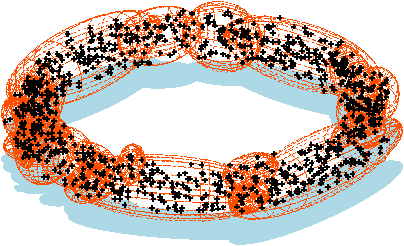
\includegraphics[width=\textwidth]{figures/multinest}
        \texttt{UltraNest}~\arxiv{2101.09604}
        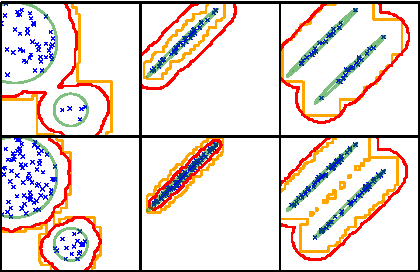
\includegraphics[width=\textwidth]{figures/radfriends}
        \texttt{nautilus}~\arxiv{2306.16923} 
        \column{0.4\textwidth}
        \texttt{PolyChord}~\arxiv{1506.00171}
        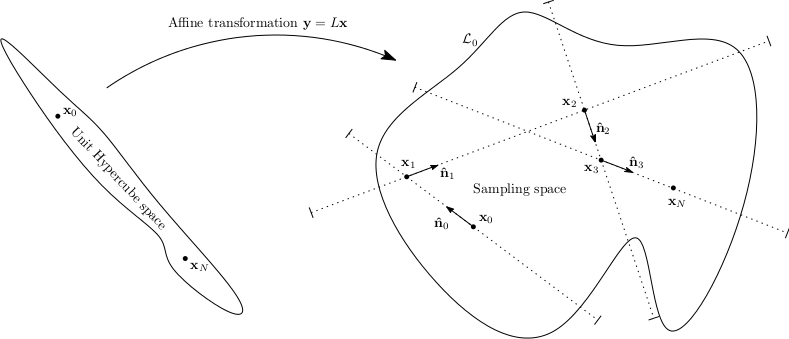
\includegraphics[width=\textwidth]{figures/polychord}
        \vfill
        \texttt{NeuralNest}~\arxiv{1903.10860}
        \begin{columns}
            \column{0.55\textwidth}
            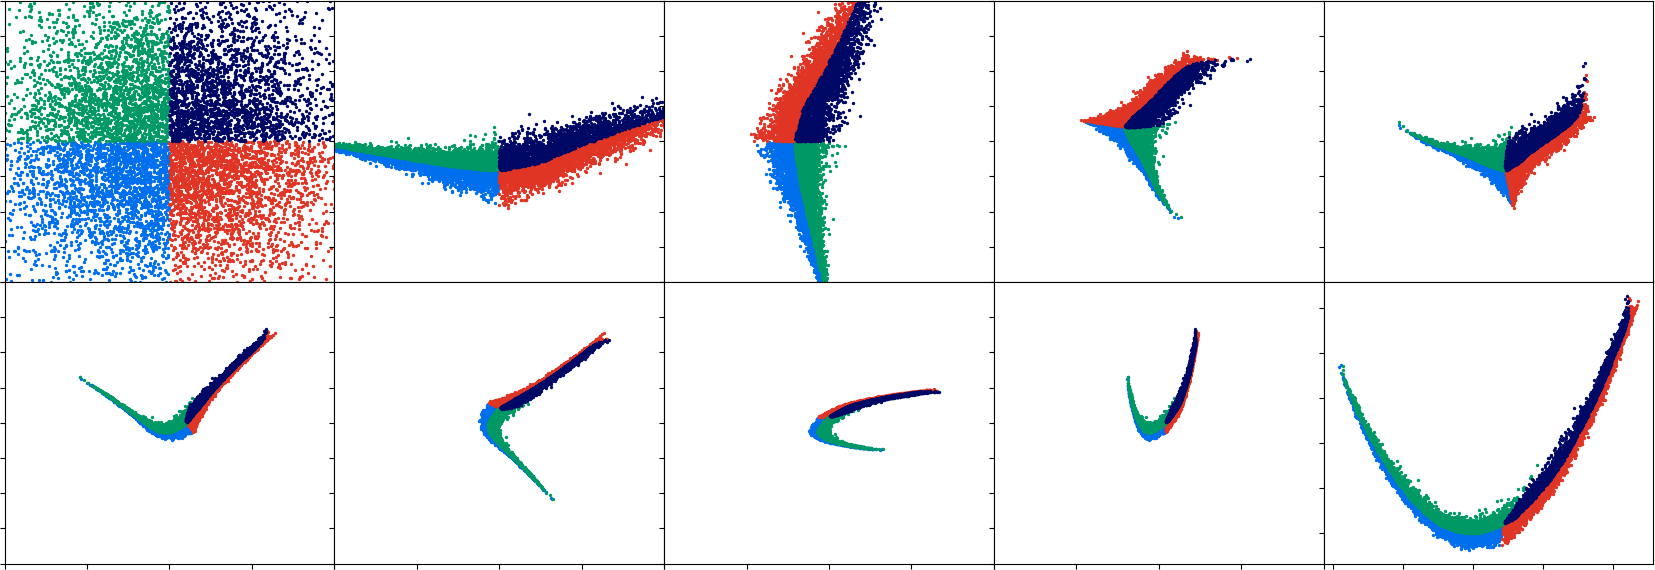
\includegraphics[width=\textwidth]{figures/rosenbrock_flow.png}
            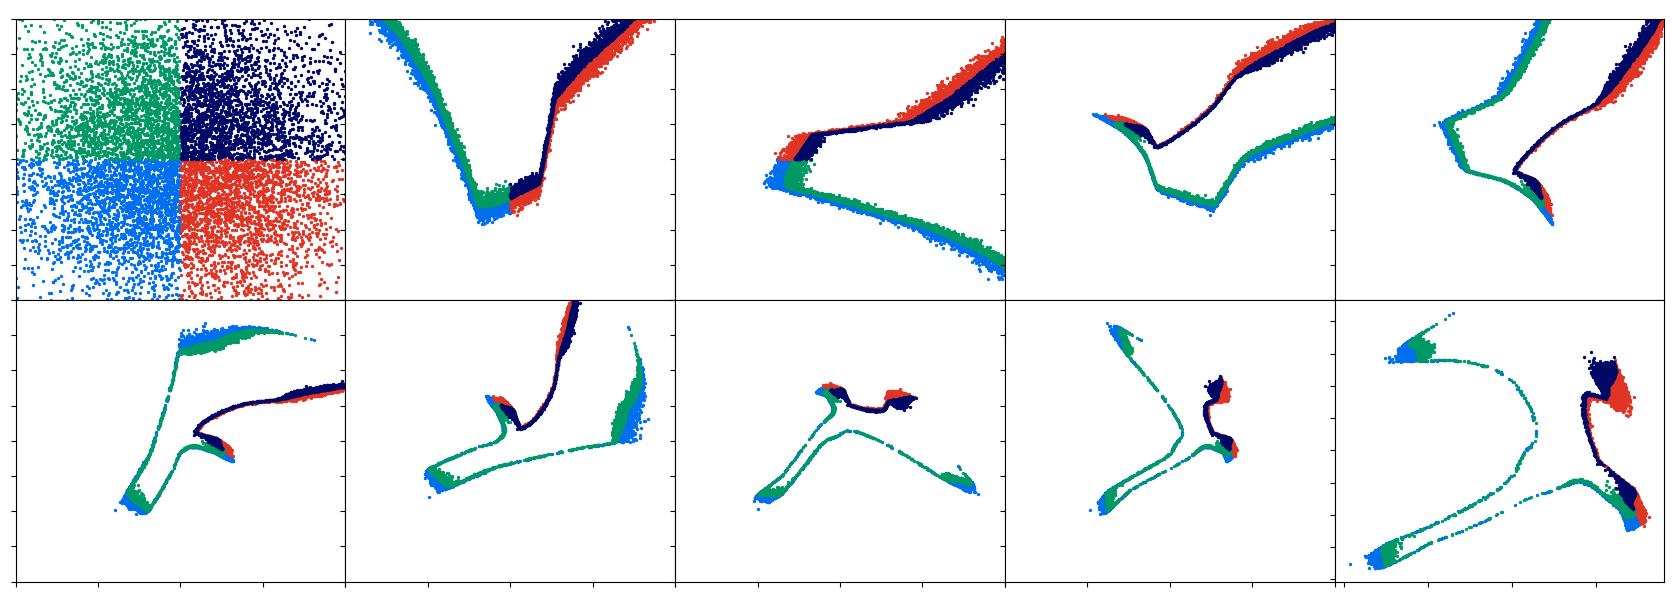
\includegraphics[width=\textwidth]{figures/himmelblau_flow.png}
            \column{0.45\textwidth}
            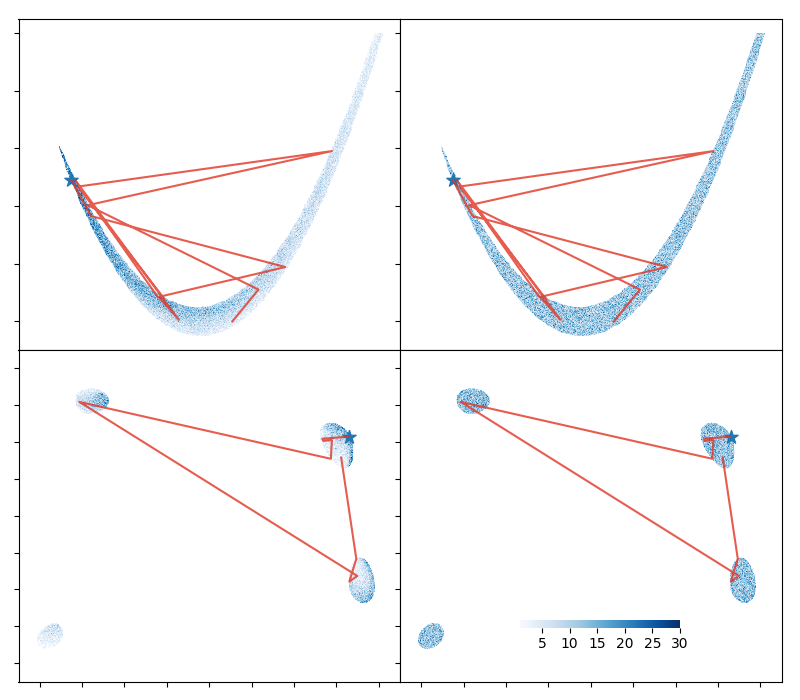
\includegraphics[width=\textwidth]{figures/chains.png}
        \end{columns}
        \texttt{nessai}~\arxiv{2102.11056} \texttt{cpnest} \texttt{nora}~\arxiv{2305.19267} \texttt{jaxns}~\arxiv{2012.15286}
        \vfill
        \column{0.3\textwidth}
        \texttt{DNest}~\arxiv{1606.03757}
        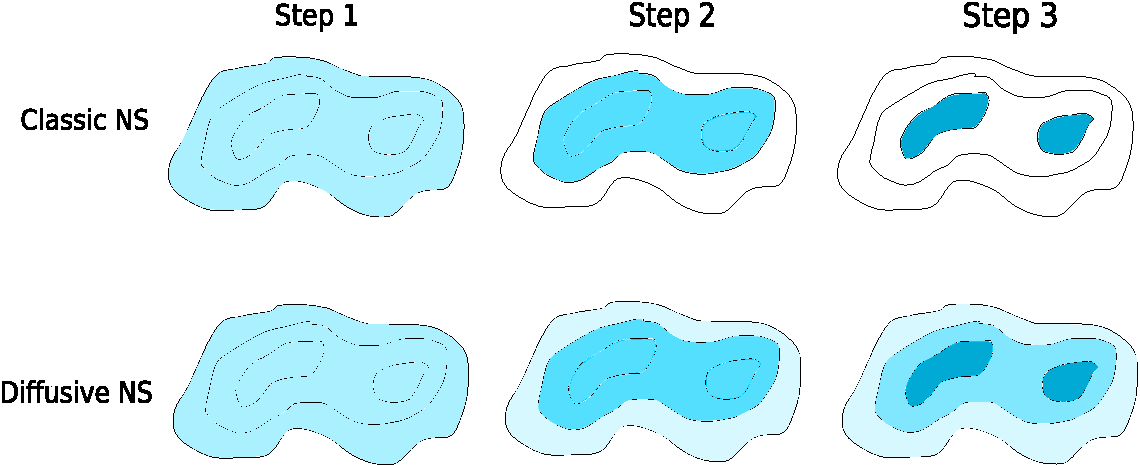
\includegraphics[width=\textwidth]{figures/dnest}
        \texttt{ProxNest}~\arxiv{2106.03646}
        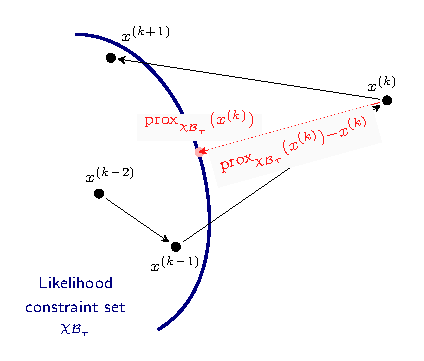
\includegraphics[width=\textwidth]{figures/proxnest_diagram}
        \texttt{dynesty}~\arxiv{1904.02180} 
        \vfill
    \end{columns}
\end{frame}

\begin{frame}
    \frametitle{Types of nested sampler}
    \begin{itemize}
        \item Broadly, most nested samplers can be split into how they create new live points.
        \item i.e. how they sample from the hard likelihood constraint $\{\theta\sim \pi : \mathcal{L}(\theta)>\mathcal{L}_* \}$.
    \end{itemize}
    \vspace{-10pt}
    \begin{columns}[t]
        \column{0.48\textwidth}
        \begin{block}{Rejection samplers}
            \begin{itemize}
                \item e.g. \texttt{MultiNest}, \texttt{UltraNest}.
\item Constructs bounding region and draws many invalid points until $\mathcal{L}(\theta)>\mathcal{L}_*$.
                \item Efficient in low dimensions, exponentially inefficient $\sim\mathcal{O}(e^{d/d_0})$ in high  $d>d_0\sim10$.
            \end{itemize}
        \end{block}
        \column{0.48\textwidth}
        \begin{block}{Chain-based samplers}
            \begin{itemize}
                \item e.g. \texttt{PolyChord}, \texttt{ProxNest}.
                \item Run Markov chain starting at a live point, generating many valid (correlated) points.
                \item Linear $\sim\mathcal{O}(d)$ penalty in decorrelating new live point from the original seed point.
            \end{itemize}
        \end{block}
    \end{columns}
    \vspace{5pt}
    \begin{itemize}
        \item Nested samplers usually come with:
            \begin{itemize}
                \item \emph{resolution} parameter $n_\text{live}$ (which improve results as $\sim\mathcal{O}(n_\text{live}^{-1/2})$.
                    \item set of \emph{reliability} parameters~\arxiv{2101.04525}, which don't improve results if set arbitrarily high, but introduce systematic errors if set too low.
                    \item e.g. \texttt{Multinest} efficiency \texttt{eff} or \texttt{PolyChord} chain length $n_\text{repeats}$.
            \end{itemize}
    \end{itemize}
\end{frame}

\begin{frame}
    \frametitle{SBI: Simulation-based inference}
    \begin{columns}
        \column{0.5\textwidth}
        \begin{itemize}
            \item What do you do if you don't know \C[2]{$\mathcal{L}(D|\theta)$}?
            \item If you have a simulator/forward model $\theta \rightarrow D$
                defines an \C[2]{\emph{implicit} likelihood~$\mathcal{L}$}.
            \item Simulator generates samples from $\C[2]{\mathcal{L}(\cdot|\theta)}$.
            \item With a prior $\C[1]{\pi}(\theta)$ can generate samples from \C[4]{joint distribution}~$\C[4]{\mathcal{J}(\theta,D)}=\C[2]{\mathcal{L}(D|\theta)}\C[1]{\pi(\theta)}$\\\hfill \emph{the ``probability of everything''}.
            \item Task of SBI is take joint~$\C[4]{\mathcal{J}}$ samples and learn \C[0]{posterior $\mathcal{P}(\theta|D)$} and \C[3]{evidence $\mathcal{Z}(D)$} \\\hfill and possibly \C[2]{likelihood $\mathcal{L}(D|\theta)$}.
            \item Present state of the art achieves this using \emph{machine learning} (neural networks).
                \begin{itemize}
                    \item My group's research tries to removes machine learning \tthref{github.com/handley-lab/lsbi}.
                \end{itemize}
        \end{itemize}
        \column{0.5\textwidth}
        \includegraphics<1>[page=1, width=\textwidth]{figures/sbi_parameter_estimation.pdf}%
        \includegraphics<2>[page=2, width=\textwidth]{figures/sbi_parameter_estimation.pdf}%
        \includegraphics<3>[page=3, width=\textwidth]{figures/sbi_parameter_estimation.pdf}%
        \includegraphics<4>[page=4, width=\textwidth]{figures/sbi_parameter_estimation.pdf}%
        \includegraphics<5>[page=5, width=\textwidth]{figures/sbi_parameter_estimation.pdf}%
        \includegraphics<6>[page=6, width=\textwidth]{figures/sbi_parameter_estimation.pdf}%
        \includegraphics<7>[page=7, width=\textwidth]{figures/sbi_parameter_estimation.pdf}%
        \includegraphics<8>[page=8, width=\textwidth]{figures/sbi_parameter_estimation.pdf}%
        \includegraphics<9>[page=9, width=\textwidth]{figures/sbi_parameter_estimation.pdf}%
        \includegraphics<10>[page=10, width=\textwidth]{figures/sbi_parameter_estimation.pdf}%
        \includegraphics<11>[page=11, width=\textwidth]{figures/sbi_parameter_estimation.pdf}%
        \includegraphics<12>[page=12, width=\textwidth]{figures/sbi_parameter_estimation.pdf}%
        \includegraphics<13>[page=13, width=\textwidth]{figures/sbi_parameter_estimation.pdf}%
        \includegraphics<14>[page=14, width=\textwidth]{figures/sbi_parameter_estimation.pdf}%
        \includegraphics<15>[page=15, width=\textwidth]{figures/sbi_parameter_estimation.pdf}%
        \includegraphics<16>[page=16, width=\textwidth]{figures/sbi_parameter_estimation.pdf}%
        \includegraphics<17>[page=17, width=\textwidth]{figures/sbi_parameter_estimation.pdf}%
        \includegraphics<18>[page=18, width=\textwidth]{figures/sbi_parameter_estimation.pdf}%
        \includegraphics<19>[page=19, width=\textwidth]{figures/sbi_parameter_estimation.pdf}%
        \includegraphics<20>[page=20, width=\textwidth]{figures/sbi_parameter_estimation.pdf}%
        \includegraphics<21>[page=21, width=\textwidth]{figures/sbi_parameter_estimation.pdf}%
    \end{columns}
\end{frame}

\begin{frame}
    \frametitle{Why SBI?}
    \begin{columns}
        \column{0.6\textwidth}
        SBI is useful because:
        \begin{enumerate}
            \item If you don't have a likelihood, you can still do inference
                \begin{itemize}
                    \item This is the usual case beyond CMB cosmology
                \end{itemize}
            \item Faster than LBI
                \begin{itemize}
                    \item emulation -- also applies to LBI in principle
                \end{itemize}
            \item No need to pragmatically encode fiducial cosmologies
                \begin{itemize}
                    \item Covariance computation implicitly encoded in simulations
                    \item Highly relevant for disentangling tensions \& systematics
                \end{itemize}
            \item Equips AI/ML with Bayesian interpretability
            \item Lower barrier to entry than LBI
                \begin{itemize}
                    \item Much easier to forward model a systematic
                    \item Emerging set of plug-and-play packages
                    \item For this reason alone, it will come to dominate scientific inference
                \end{itemize}
        \end{enumerate}
        \column{0.4\textwidth}
        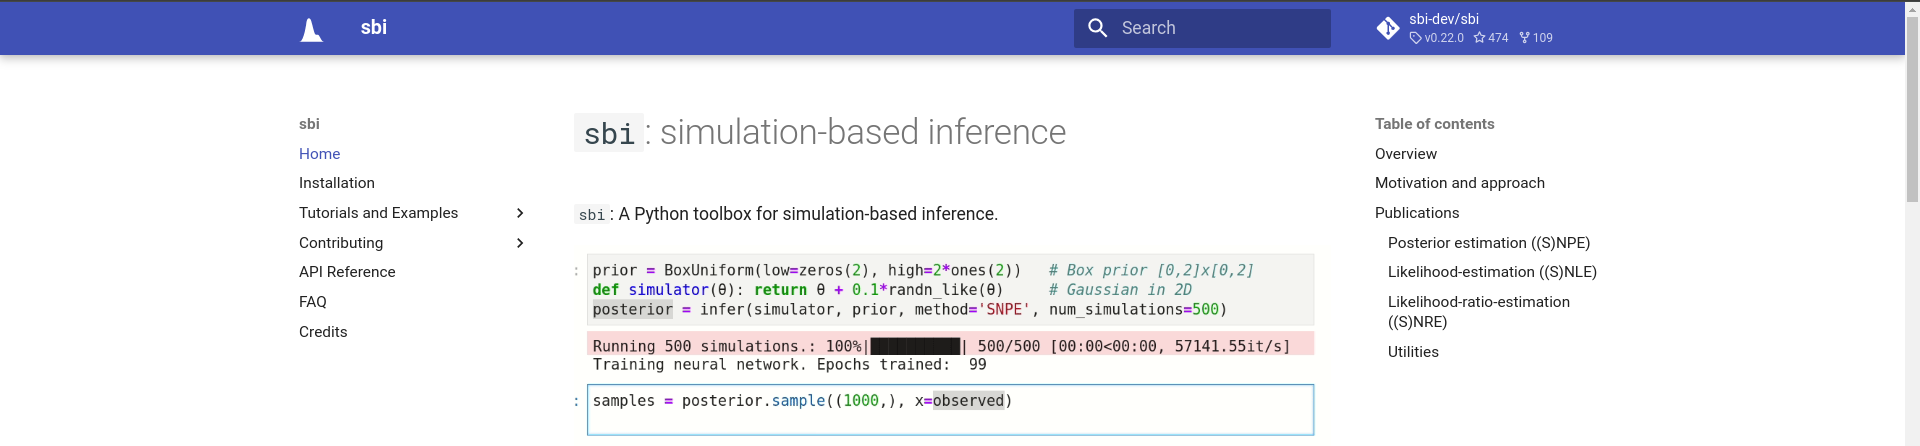
\includegraphics[width=\textwidth]{figures/sbi_screenshot}
        \href{https://github.com/sbi-dev}{github.com/sbi-dev}
        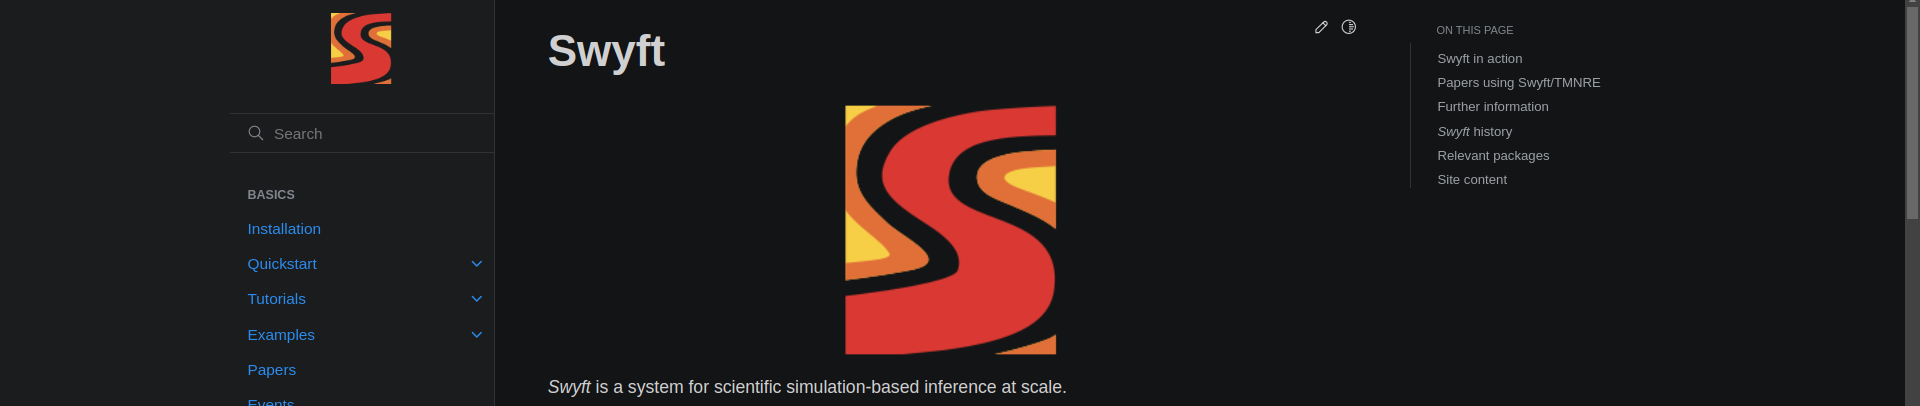
\includegraphics[width=\textwidth]{figures/swyft_screenshot}
        \href{https://github.com/undark-lab/swyft}{github.com/undark-lab/swyft}
        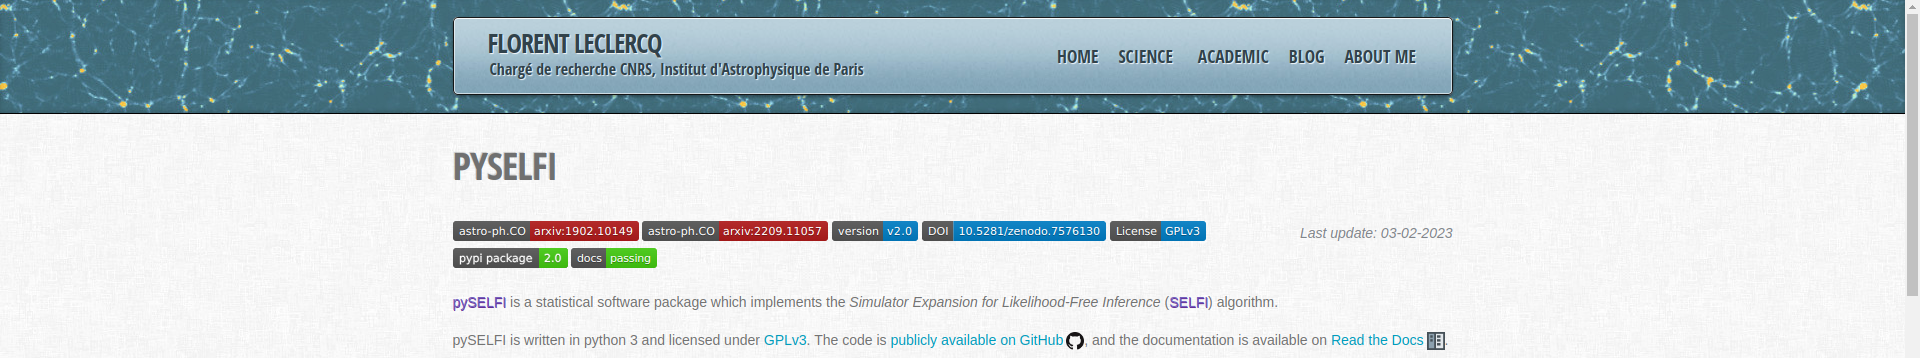
\includegraphics[width=\textwidth]{figures/selfi_screenshot}
        \href{https://github.com/florent-leclercq/pyselfi}{github.com/florent-leclercq/pyselfi}
        
\includegraphics[width=\textwidth]{figures/delfi_screenshot}
        \href{https://github.com/justinalsing/pydelfi}{github.com/justinalsing/pydelfi}
    \end{columns}
\end{frame}

\begin{frame}
    \frametitle{SBI in astrophysics}
    \begin{columns}
        \column{0.4\textwidth}
        \begin{itemize}
            \item 2024 has been the year it has started to be applied to real data.
            \item Mostly for weak lensing
            \item However: SBI requires mock data generation code
            \item Most data analysis codes were built before the generative paradigm.
            \item It's still a lot of work to upgrade cosmological likelihoods  to be able to do this (e.g.\ \texttt{plik} \& \texttt{camspec}).
        \end{itemize}
        \column{0.3\textwidth}
        
\includegraphics[width=\textwidth]{figures/sbi_papers/clusters.pdf}
        \vspace{10pt}\\
        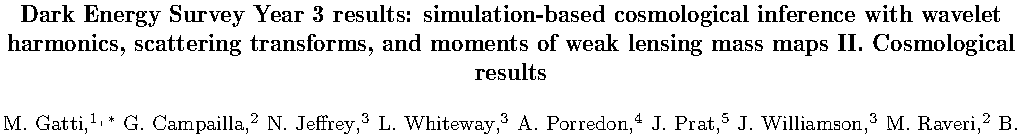
\includegraphics[width=\textwidth]{figures/sbi_papers/des.pdf}
        \vspace{10pt}\\
        
\includegraphics[width=\textwidth]{figures/sbi_papers/gw.pdf}
        \vspace{10pt}\\
        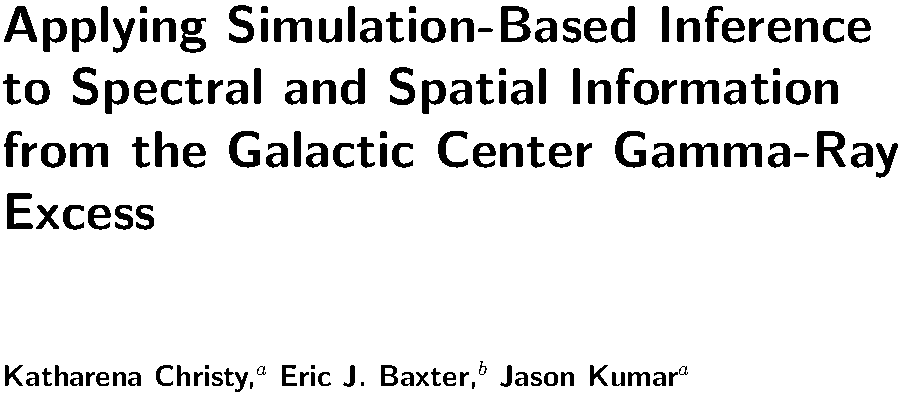
\includegraphics[width=\textwidth]{figures/sbi_papers/center.pdf}
        \column{0.3\textwidth}
        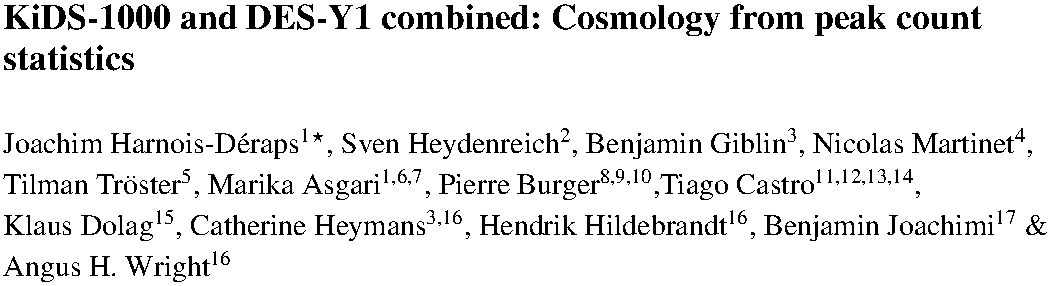
\includegraphics[width=\textwidth]{figures/sbi_papers/kidsdes.pdf}
        \vspace{10pt}\\
        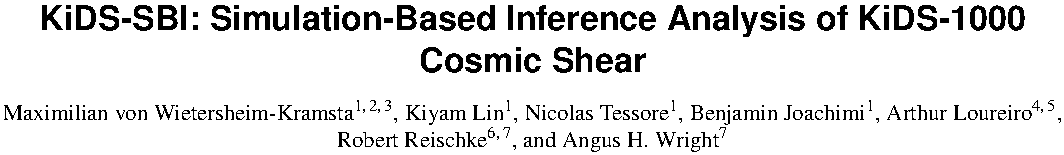
\includegraphics[width=\textwidth]{figures/sbi_papers/kids.pdf}
        \vspace{10pt}\\
        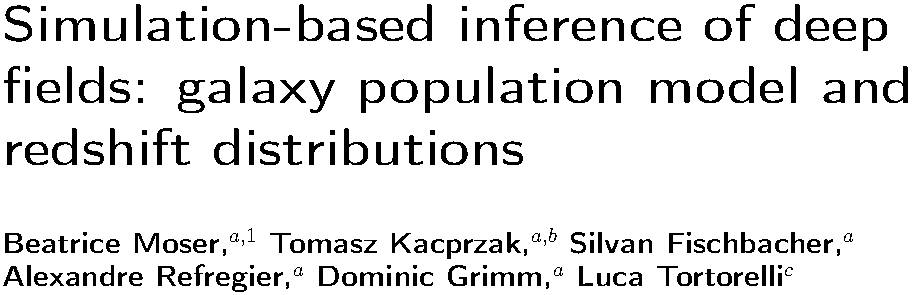
\includegraphics[width=\textwidth]{figures/sbi_papers/population.pdf}
        \vspace{10pt}\\
        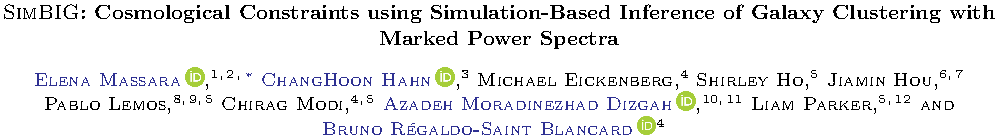
\includegraphics[width=\textwidth]{figures/sbi_papers/simbig.pdf}
    \end{columns}
\end{frame}

\begin{frame}
    \frametitle{Neural Ratio Estimation}
    \begin{columns}
        \column{0.5\textwidth}
        \begin{itemize}
            \item SBI flavours: {\small \hfill\tthref{github.com/sbi-dev/sbi}}
                {\small
                    \begin{description}
                        \item[NPE] Neural posterior estimation
                        \item[NLE] Neural likelihood estimation
                        \item[NJE] Neural joint estimation
                        \item[NRE] Neural ratio estimation
                    \end{description}
                }
            \item NRE recap:
                \begin{enumerate}
                    \item Generate joint samples $(\theta,D)\sim\C[4]{\mathcal{J}}$
                        \label{step:joint}
                        \begin{itemize}
                            \item \textit{straightforward if you have a simulator:\\ $\theta\sim\C[1]{\pi(\cdot)}$, $D\sim\C[2]{\mathcal{L}(\cdot|\theta)}$}
                        \end{itemize}
                    \item Generate separated samples $\theta\sim\C[1]{\pi}$, $D\sim\C[3]{\mathcal{Z}}$\label{step:sep}
                        \begin{itemize}
                            \item \textit{aside: can shortcut step~\ref{step:sep} by scrambling the $(\theta,D)$ pairings from step~\ref{step:joint}}
                        \end{itemize}
                    \item Train probabilistic classifier $p$ to distinguish whether $(\theta,D)$ came from $\C[4]{\mathcal{J}}$ or $\C[1]{\pi}\times\C[3]{\mathcal{Z}}$.
                    \item $\frac{p}{1-p} = \C[5]{r} = \frac{P(\theta,D)}{P(\theta)P(D)} 
                        =
                        \frac{\C[4]{\mathcal{J}}}{\C[1]{\pi}\times\C[3]{\mathcal{Z}}} = \frac{\C[2]{\mathcal{L}}}{\C[3]{\mathcal{Z}}} = \frac{\C[0]{\mathcal{P}}}{\C[1]{\pi}}$.
                    \item Use ratio $\C[5]{r}$ for parameter estimation $\C[0]{\mathcal{P}} = \C[5]{r}\C[1]\times {\pi}$
                \end{enumerate}
        \end{itemize}
        \column{0.5\textwidth}
        \only<1|handout:0>{
            \begin{tikzpicture}[node distance=1cm, every neuron/.style={circle, draw, minimum size=1cm},]
                \node[every neuron/.try] (j2)  {};
                \node[every neuron/.try, above left = 0cm and 0.5cm of j2] (theta) { $\theta$};
                \node[every neuron/.try, below left = 0cm and 0.5cm of j2] (D) { $D$};
                \node[every neuron/.try, above = 0.5cm of j2] (j1) {};
                \node[every neuron/.try, below = 0.5cm of j2] (j3) {};
                \node[every neuron/.try, above right = 0cm and 0.5cm of j2] (h1) {};
                \node[every neuron/.try, below right = 0cm and 0.5cm of j2] (h2) {};
                \node[every neuron/.try, right = 1.3cm of j2] (p) { $p$};
                \node[every neuron/.try, right = 0.5cm of p] (logr) { $\C[5]{r}$};
                \draw[-] (theta) -- (j1);
                \draw[-] (D) -- (j1);
                \draw[-] (theta) -- (j2);
                \draw[-] (D) -- (j2);
                \draw[-] (theta) -- (j3);
                \draw[-] (D) -- (j3);
                \draw[-] (j1) -- (h1);
                \draw[-] (j1) -- (h2);
                \draw[-] (j2) -- (h1);
                \draw[-] (j2) -- (h2);
                \draw[-] (j3) -- (h1);
                \draw[-] (j3) -- (h2);
                \draw[-] (h1) -- (p);
                \draw[-] (h2) -- (p);
                \draw[-] (p) -- (logr);
                \node[below =0.5cm of logr] {\includegraphics[page=22, width=0.5\textwidth]{figures/sbi_parameter_estimation.pdf}};
            \end{tikzpicture}
        }
        \only<2>{
            \begin{exampleblock}{Bayesian proof}
                \begin{itemize}
                    \item Let $M_{\C[4]{\mathcal{J}}}$: $(\theta,D)\sim\C[4]{\mathcal{J}}$, $M_{\C[1]{\pi}\C[3]{\mathcal{Z}}}$: $(\theta,D)\sim\C[1]{\pi}\times\C[3]{\mathcal{Z}}$
                    \item Classifier gives
                        ${p(\theta,D) = P(M_{\C[4]{\mathcal{J}}}|\theta,D) = 1- P(M_{\C[1]{\pi}\C[3]{\mathcal{Z}}}|\theta,D)}$
                    \item Bayes theorem then shows
                        ${\frac{p}{1-p}=\frac{P(M_{\C[4]{\mathcal{J}}}|\theta,D)}{P(M_{\C[1]{\pi}\C[3]{\mathcal{Z}}}|\theta,D)} = \frac{P(\theta,D|M_{\C[4]{\mathcal{J}}})P(M_{\C[4]{\mathcal{J}}})}{P(\theta,D|M_{\C[1]{\pi}\C[3]{\mathcal{Z}}})P(M_{\C[1]{\pi}\C[3]{\mathcal{Z}}})} = 
                        \frac{\C[4]{\mathcal{J}}}{\C[1]{\pi}\C[3]{\mathcal{Z}}}}$, \\
                        where we have assumed 
                        \begin{itemize}
                            \item $P(M_{\C[4]{\mathcal{J}}}) = P(M_{\C[1]{\pi}\C[3]{\mathcal{Z}}})$,
                        \end{itemize}
                        and by definition
                        \begin{itemize}
                            \item $\C[4]{\mathcal{J}(\theta,D)} = P(\theta,D|M_{\C[4]{\mathcal{J}}})$
                            \item $\C[1]{\pi(\theta)}\C[3]{\mathcal{Z}(D)} = P(\theta,D|M_{\C[1]{\pi}\C[3]{\mathcal{Z}}})$.
                        \end{itemize}
                \end{itemize}
            \end{exampleblock}
        }
        \only<3|handout:0>{
            \begin{block}{Why I like NRE}
                \begin{itemize}
                    \item The link between classification and inference is profound.
                    \item Density estimation is hard -- Dimensionless $r$ divides out the hard-to-calculate parts.
                \end{itemize}
            \end{block}
            \begin{block}{Why I don't like NRE}
                \begin{itemize}
                    \item Practical implementations require marginalisation~\arxiv{2107.01214}, or autoregression~\arxiv{2308.08597}.
                    \item Model comparison and parameter estimation are separate~\arxiv{2305.11241}.
                \end{itemize}
            \end{block}
        }
    \end{columns}
\end{frame}

\begin{frame}
    \frametitle{Marginal inference}
    \student{harry_bevins}{Harry Bevins}{PhD$\to$JRF}
    \begin{columns}
        \column{0.5\textwidth}
        \begin{itemize}
            \item Many cosmological likelihoods come with nuisance parameters that have limited relevance for onward inference.
            \item Notation: \only<1>{CMB cosmology} \only<2>{GW cosmology}
                \begin{itemize}
                    \item[$\mathcal{L}$] Likelihood \hfill (e.g. \only<1>{\texttt{plik}}\only<2>{LAL}),
                    \item[$D$] Data \hfill (e.g. \only<1>{CMB}\only<2>{GW170817}),
                    \item[$\theta$] Cosmological parameters \hfill (e.g. \only<1>{$\Omega_m$}, $H_0$\ldots),
                    \item[$\alpha$] Nuisance parameters \hfill (e.g. \only<1>{$A_\text{planck}$}\only<2>{$m_1$, $m_2$}\ldots),
                    \item[$M$] Model \hfill (e.g. $\Lambda$CDM).
                \end{itemize}
            \item Some marginal statistics (e.g. marginal means, posteriors\ldots) are easy to compute.
            \item More machinery is needed for e.g. nuisance marginalised likelihoods and marginal KL divergences $\mathcal{D}_\text{KL}$.
        \end{itemize}
        \column{0.5\textwidth}
        \vspace{10pt}
        \includegraphics<1>{figures/planck_2018_plik.pdf}%
        \includegraphics<2>[width=\textwidth]{figures/standardsirens}
        \includegraphics<2>[width=\textwidth]{figures/graveyard}
    \end{columns}
\end{frame}

\begin{frame}
    \frametitle{Nuisance marginalised likelihoods: Theory {\small\arxiv{2207.11457}}}
    \student{harry_bevins}{Harry Bevins}{PhD$\to$JRF}
    \begin{columns}[t]
        \column{0.5\textwidth}
        \begin{itemize}
            \item Bayes theorem
                \begin{align}
                    \C[2]{\mathcal{L}}(\theta,\alpha) 
                    \times 
                    \C[1]{\pi}(\theta,\alpha) &= 
                    \C[0]{\mathcal{P}}(\theta,\alpha)
                    \times
                    \C[3]{\mathcal{Z}}\\
                    \C[2]{\text{Likelihood}}
                    \times
                    \C[1]{\text{Prior}}
                    &=
                    \C[0]{\text{Posterior}}
                    \times
                    \C[3]{\text{Evidence}}
                    \nonumber
                \end{align}
                \small{$\alpha$: nuisance parameters, $\theta$: cosmo parameters.}
            \item Marginal Bayes theorem
                \begin{equation}
                    \C[2]{\mathcal{L}}(\theta) 
                    \times 
                    \C[1]{\pi}(\theta) = 
                    \C[0]{\mathcal{P}}(\theta)
                    \times
                    \C[3]{\mathcal{Z}}
                \end{equation}
            \item Non-trivially gives \textbf{nuisance-free likelihood}
                \begin{equation}
                    \boxed{
                        \C[2]{\mathcal{L}}(\theta) 
                        = 
                        \frac{
                            \C[0]{\mathcal{P}}(\theta)
                            \C[3]{\mathcal{Z}}
                        }{
                            \C[1]{\pi}(\theta)
                        }
                    }
                    =
                    \frac{
                        \int \C[2]{\mathcal{L}}(\theta,\alpha) \C[1]{\pi}(\theta,\alpha) d{\alpha}
                    }
                    {
                        \int \C[1]{\pi}(\theta,\alpha) d{\alpha}
                    }
                \end{equation}
        \end{itemize}
        \column{0.5\textwidth}
        \textbf{Key properties}
        \begin{itemize}
            \item Given datasets $A$ and $B$, each with own nuisance parameters $\alpha_A$ and $\alpha_B$:
            \item If you use $\mathcal{L}_A(\theta)$, you get the same (marginal) posterior and evidence if you had run with nuisance parameters $\alpha_A$ (ditto $B$).
            \item If you run inference on $\mathcal{L}_A(\theta)\times\mathcal{L}_B(\theta)$, you get the same (marginal) posterior and evidence if you had run with all nuisance parameters $\alpha_A$, $\alpha_B$ on.
            \item[] \textit{(weak marginal consistency requirements on joint $\pi(\theta,\alpha_A,\alpha_B)$ and marginal priors)}
        \end{itemize}
    \end{columns}
\end{frame}

\begin{frame}
    \frametitle{Nuisance marginalised likelihoods: Practice~{\small\arxiv{2205.12841}}}
    \student{harry_bevins}{Harry Bevins}{PhD$\to$JRF}
    \begin{columns}
        \column{0.6\textwidth}
        \begin{columns}
            \column{0.3\textwidth}
            \[
                \boxed{
                    \C[2]{\mathcal{L}}(\theta) 
                    = 
                    \frac{
                        \C[0]{\mathcal{P}}(\theta)
                        \C[3]{\mathcal{Z}}
                    }{
                        \C[1]{\pi}(\theta)
                    }
                }
            \]
            \column{0.7\textwidth}
            \begin{itemize}
                \item To compute the nuisance marginalised likelihood, need:
                    \begin{enumerate}
                        \item Bayesian evidence $\C[3]{\mathcal{Z}}$
                        \item Marginal prior and posterior \textbf{densities}
                    \end{enumerate}
            \end{itemize}
        \end{columns}
        \begin{enumerate}
            \item Bayesian evidence $\C[3]{\mathcal{Z}}$:                              g
                \begin{itemize}
                    \item Nested sampling
                    \item Parallel tempering (pocomc, ptmcmc)
                    \item Sequential Monte Carlo (SMC)
                    \item MCEvidence
                \end{itemize}
            \item Marginal prior $\C[1]{\pi}(\theta)$ and posterior $\C[0]{\mathcal{P}}(\theta)$ densities:
                \begin{itemize}
                    \item Histograms of samples
                    \item Kernel density estimation
                    \item Normalising flows / Diffusion models
                    \item \ldots
                \end{itemize}
        \end{enumerate}
        \begin{itemize}
            %\item Combination termed \texttt{margarine} \arxiv{2205.12841}
            \item Emulators usually much faster than original likelihoods
            \item \texttt{margarine}: PyPI, \href{https://github.com/htjb/margarine}{github.com/htjb/margarine}
        \end{itemize}
        \column{0.4\textwidth}
        \begin{tikzpicture}[
                rednode/.style={rectangle, draw=red!60, fill=red!5, very thick, minimum size=5mm},
                bluenode/.style={rectangle, draw=blue!60, fill=blue!5, very thick, minimum size=5mm},
                greennode/.style={rectangle, draw=green!60, very thick, minimum size=5mm},
                node distance=0.5cm,
                remember picture, overlay
            ]
            \node<1->[bluenode, xshift=0.5\textwidth, yshift=-0.25\textwidth](likelihood) at (current page.north)  {$ \mathcal{L}(\theta,\alpha)$};
            \node<1->[bluenode, right = of likelihood.east](prior) {$ \pi(\theta,\alpha)$};
            \coordinate<1-> (likelihoodprior) at ($(likelihood.south)!0.5!(prior.south)$);
            \node<2->[rednode, below = of likelihoodprior](nestedsampling) {Nested Sampling};
            \draw<2->[->](likelihood.south) -- (likelihood|-nestedsampling.north);
            \draw<2->[->](prior.south) -- (prior|-nestedsampling.north);
            \node<3->[bluenode, below = of nestedsampling](posterior) {$ \{\theta,\alpha\}_\mathcal{P}$};
            \draw<3->[->](nestedsampling.south-|posterior) -- (posterior.north);
            \node<4->[bluenode, left = of posterior.west](evidence) {$ \mathcal{Z}$};
            \draw<4->[->](nestedsampling.south-|likelihood) -- (evidence.north);
            \node<5->[bluenode, right = of posterior.east](priorSamples) {$ \{\theta,\alpha\}_\pi$};
            \draw<5->[->](nestedsampling.south-|prior) -- (priorSamples.north);
            \coordinate<5-> (posteriorprior) at ($(posterior.south)!0.5!(priorSamples.south)$);
            \node<6->[rednode, below = of posteriorprior](margarine)  {Density Estimation};
            \draw<6->[->](posterior.south) -- (margarine.north-|posterior.east);
            \draw<6->[->](priorSamples.south) -- (margarine.north-|priorSamples.west);
            \node<7->[bluenode, below = of posterior|-margarine.south](marginalPosterior) {$ \mathcal{P}(\theta)$};
            \draw<7->[->](margarine.south-|marginalPosterior.east) -- (marginalPosterior.north);
            \node<8->[bluenode, below = of marginalPosterior.south-|margarine.south-|priorSamples](marginalPrior) {$ \pi(\theta)$};
            \draw<8->[->](margarine.south-|priorSamples.west) -- (marginalPrior.north);
            \node<9->[bluenode, below = of marginalPosterior](marginalLikelihood) {$ \mathcal{L}(\theta)$};
            \draw<9->[->](evidence.south) -- (marginalLikelihood.west);
            \draw<9->[->](marginalPosterior.south) -- (marginalLikelihood.north);
            \draw<9->[->](marginalPrior.west) -- (marginalLikelihood.east);
            \node<10->[greennode,behind path,fit=(nestedsampling) (marginalPosterior) (priorSamples) (evidence),] {};

        \end{tikzpicture}
    \end{columns}
\end{frame}

\begin{frame}
    \frametitle{Nuisance marginalised likelihoods: Example uses}
    \student{ming_yang}{Ming Yang}{MSci}
    \begin{itemize}
        \item Library of pre-trained bijectors to be used as priors/emulators/nuisance marginalised likelihoods (DiRAC allocation \texttt{unimpeded})
        \item e.g. easy to apply a \textit{Planck}/DES/HERA/JWST prior or likelihood to your existing MCMC chains without needing to install the whole cosmology machinery.
        \item Hierarchical modelling:
            \begin{itemize}
                \item Usually, have $N$ objects, each with nuisance parameters $\alpha_i$, and shared parameters of interest $\theta$.
                \item Likelihood $\C[2]{\mathcal{L}}(\{D_i\}|\theta,\{\alpha_i\}) = \prod_i^N \C[2]{\mathcal{L}}_i(D_i|\theta,\alpha_i)$ has  $N\times \texttt{len}(\alpha_i) + \texttt{len}(\theta)$ parameters
                \item Instead, break problem down into $N$ runs on $\texttt{len}(\theta) + \texttt{len}(\alpha_i)$ parameters, and one final one on $\texttt{len}(\theta)$ parameters, using nuisance marginal likelihoods $\mathcal{L}_i(\theta)$.
                \item In addition to computational tractability, also can perform model comparison with nuisance marginalised likelihoods.
            \end{itemize}
    \end{itemize}
\end{frame}

\begin{frame}
    \frametitle{The scaling frontier of nested sampling}
    \student{zixiao_hu}{Zixiao Hu}{MSci 2023}
    \begin{columns}[t]
        \column{0.47\textwidth}
        \begin{block}{How fast in nested sampling?}
            \[ \boxed{T = T_{\C[2]{\mathcal{L}}} \times n_\text{live} \times \mathcal{D}_\text{KL} \times f_\text{sampler}} \]
        \end{block}
        \column{0.43\textwidth}
        \begin{block}{How accurate is nested sampling?}
            \[ \boxed{\sigma(\log\C[3]{\mathcal{Z}}) \approx \sqrt{\mathcal{D}_\text{KL}/n_\text{live}}} \]
        \end{block}
    \end{columns}
    \vspace{10pt}
    \begin{columns}[t]
        \column{0.5\textwidth}
        in $d$ dimensional parameter space:
        \begin{description}
\item[$T_{\C[2]{\mathcal{L}}}$:] likelihood eval time \hfill$\sim\mathcal{O}(d)$
            \item[$n_\text{live}$:] number of live points\hfill$\sim\mathcal{O}(d)$
            \item[$\mathcal{D}_\text{KL}$:] KL divergence from prior to posterior $\approx\log{V_{\C[1]{\pi}}}/{V_{\C[0]{\mathcal{P}}}}$ \hfill$\sim\mathcal{O}(d)$
            \item[$f_\text{sampler}$:] efficiency of point generation \\ region$\sim\mathcal{O}(e^{d/d_0})$ or path$\sim\mathcal{O}(d)$
        \end{description}
        \column{0.5\textwidth}
        \begin{itemize}
            \item Algorithmically improving $f_\text{sampler}$ is only a fraction of the story!
            \item $\mathcal{D}_\text{KL}$ appears twice, so improvements here are quadratically important.
            \item Gradients give you $d$ more information.
        \end{itemize}
    \end{columns}\vspace{10pt}
    \begin{itemize}
        \item $T\sim\mathcal{O}(d^4)$ whilst polynomial is far from ideal, athough progress can be made on all fronts.
    \end{itemize}
\end{frame}

\begin{frame}
    \frametitle{Accelerated nested sampling with beta flows}
    \student{metha_prathaban}{Metha Prathaban}{PhD}
    \begin{columns}
        \column{0.5\textwidth}
    \begin{itemize}
            \item For constant ``run quality'' $\sigma$, 
            \begin{gather*} 
                {\scriptstyle
                    T = T_{\C[2]{\mathcal{L}}} \times n_\text{live} \times \mathcal{D}_\text{KL} \times f_\text{sampler}, \quad
\sigma \approx \sqrt{\mathcal{D}_\text{KL}/n_\text{live}} }
    \\
\Rightarrow\boxed{T = T_{\C[2]{\mathcal{L}}} \times \sigma \times \mathcal{D}_\text{KL}^2 \times f_\text{sampler}} 
        \end{gather*}
            so if you can reduce the KL divergence, then quadratic gains to be made
        \item This can be crudely achieved by choosing a narrower prior $\pi^*$ and then correcting the evidence ${\mathcal{Z} = \mathcal{Z}^* \frac{V_{\pi}^*}{V_\pi}}$ (REACH~\arxiv{2210.07409})
        \item This can be made more sophisticated with \texttt{SuperNest}~\arxiv{2212.01760} \& posterior repartitioning
        \item Recent application to gravitational waves by Metha Prathaban~Ongoing work with\arxiv{2411.17663}.
    \end{itemize}
        \column{0.5\textwidth}
        \vspace{8pt}
        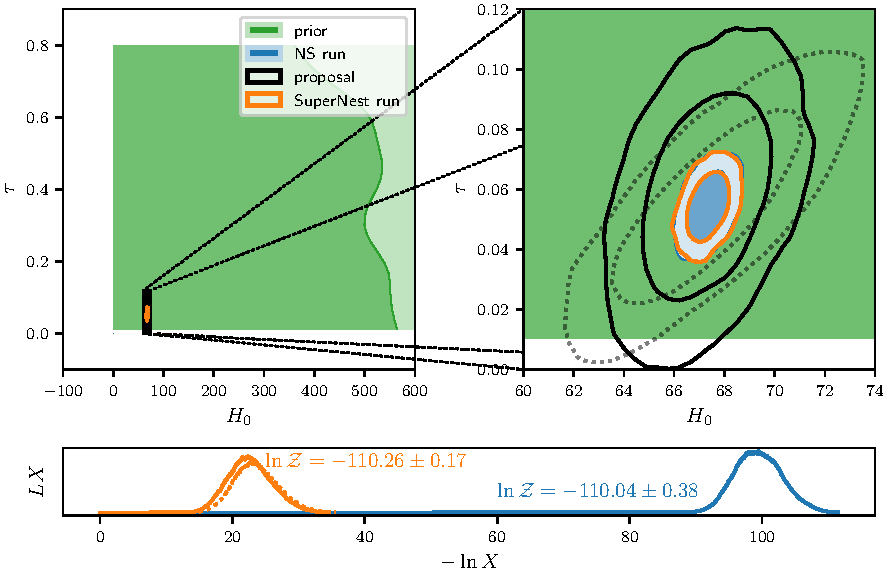
\includegraphics[width=\textwidth]{figures/supernest.pdf}
    \end{columns}
\end{frame}


\begin{frame}[fragile]
    \frametitle{Jax-based nested samplers}
    \student{david_yallup}{David Yallup}{PDRA}
    \begin{itemize}
        \item \textbf{very} recent work over the past month
        \item Have implemented a nested slice sampler in \texttt{blackjax}~[\textcolor{C0}{\texttt{\href{https://github.com/blackjax-devs/blackjax/pull/755}{\#755}}}]
\begin{lstlisting}[language=Python]
pip install git+https://github.com/handley-lab/blackjax@nested_sampling
import blackjax.ns.adaptive\end{lstlisting}
        \item parallelised over \texttt{vmap}ped likelihood \& prior evaluations
        \item Plugs into \texttt{jim}~\arxiv{kazewong/jim} and \texttt{ripple}~\arxiv{2302.05329}
        \item interested in finding use-cases for such a sampler this week
        \item Also interested in understanding current limitations/strengths of $\texttt{jax}$/GPU GW programming
    \end{itemize}
\end{frame}

\begin{frame}
    \frametitle{Conclusions}
    \framesubtitle{\tthref{github.com/handley-lab}}
    \tikz[overlay,remember picture]
        \node[anchor=north east] (A) at ($(current page.north east)+(0,0)$) {
        
\includegraphics[width=0.08\textheight]{people/adam_ormondroyd.jpg}%
        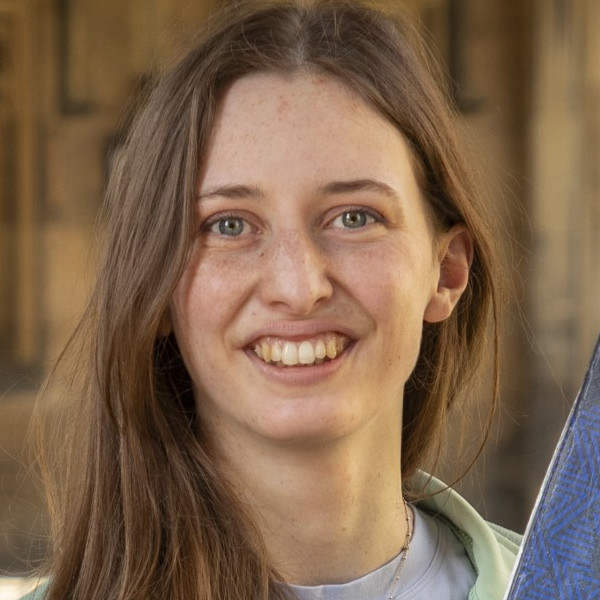
\includegraphics[width=0.08\textheight]{people/charlotte_priestley.jpg}%
        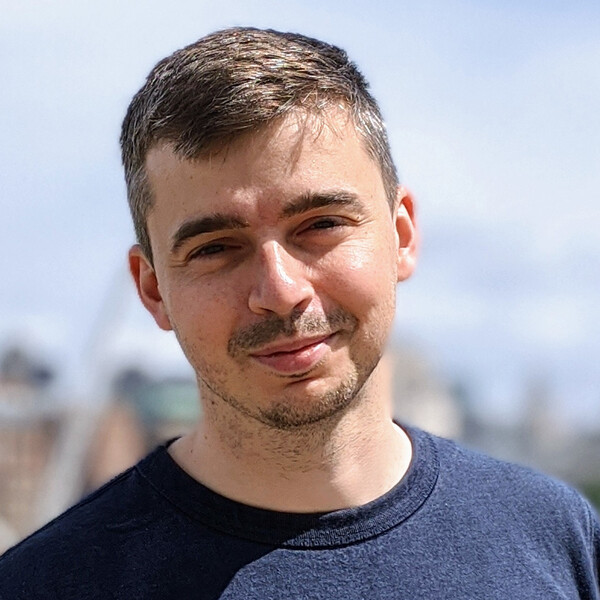
\includegraphics[width=0.08\textheight]{people/david_yallup.jpg}%
        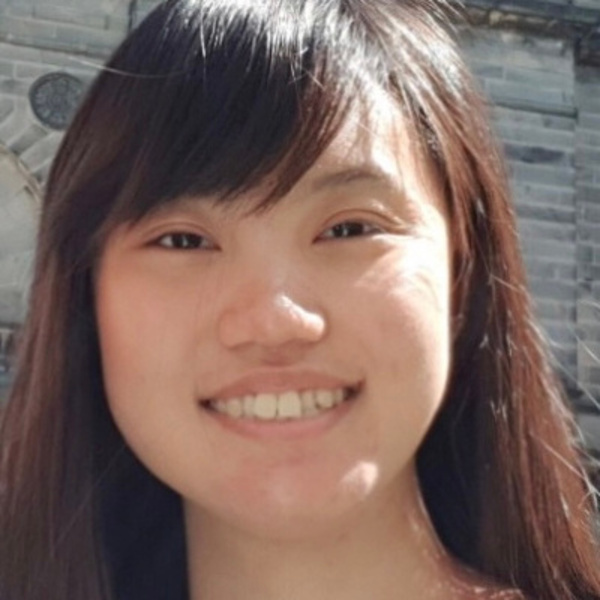
\includegraphics[width=0.08\textheight]{people/dily_ong.jpg}%
        
\includegraphics[width=0.08\textheight]{people/george_carter.jpg}%
        
\includegraphics[width=0.08\textheight]{people/harry_bevins.jpg}%
        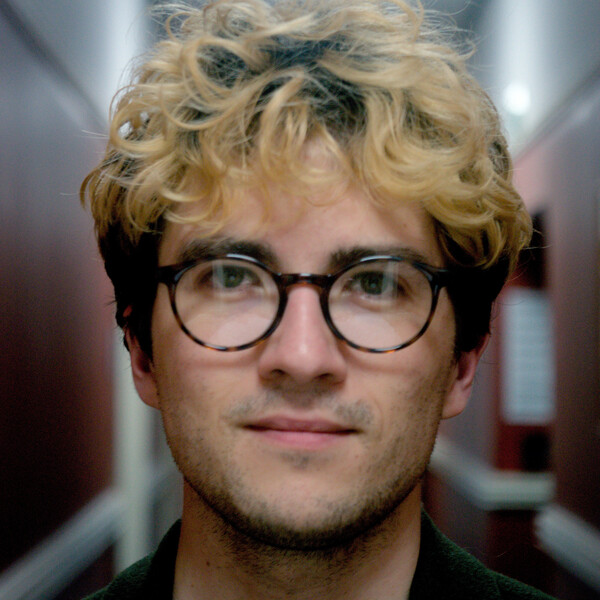
\includegraphics[width=0.08\textheight]{people/harvey_williams.jpg}%
        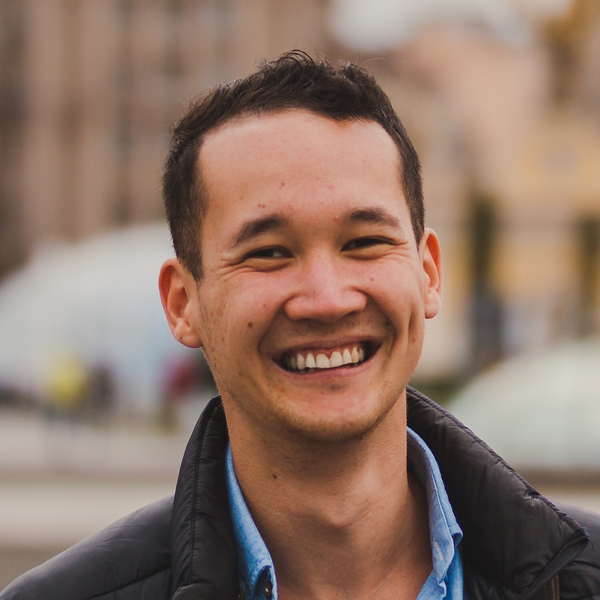
\includegraphics[width=0.08\textheight]{people/kilian_scheutwinkel.jpg}%
        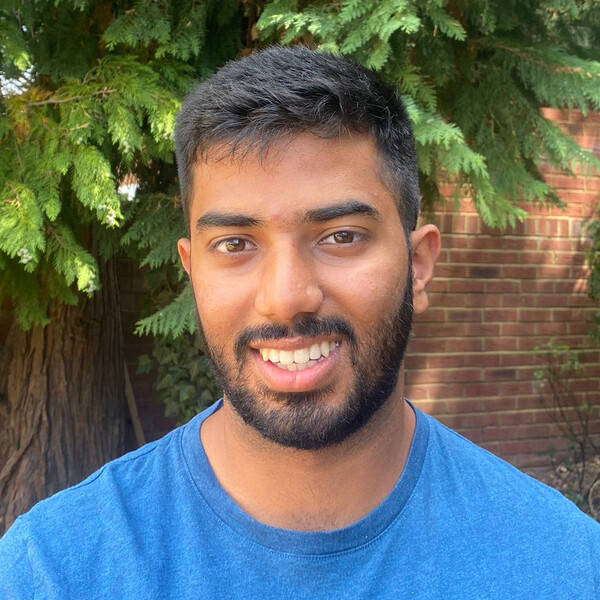
\includegraphics[width=0.08\textheight]{people/krish_nanavati.jpg}%
        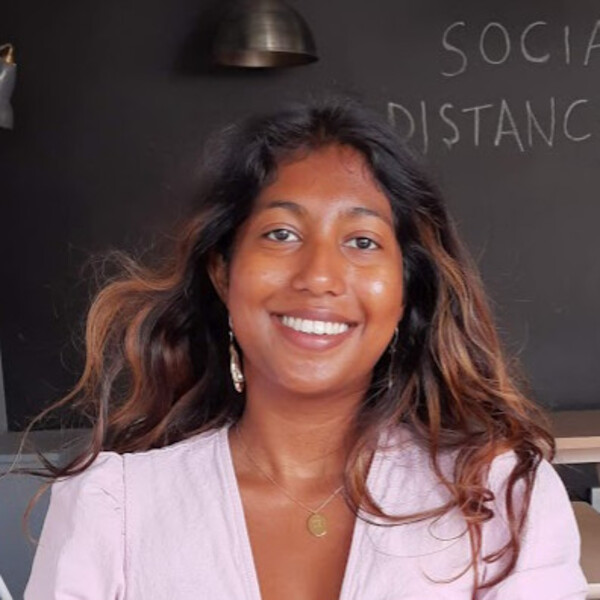
\includegraphics[width=0.08\textheight]{people/metha_prathaban.jpg}%
        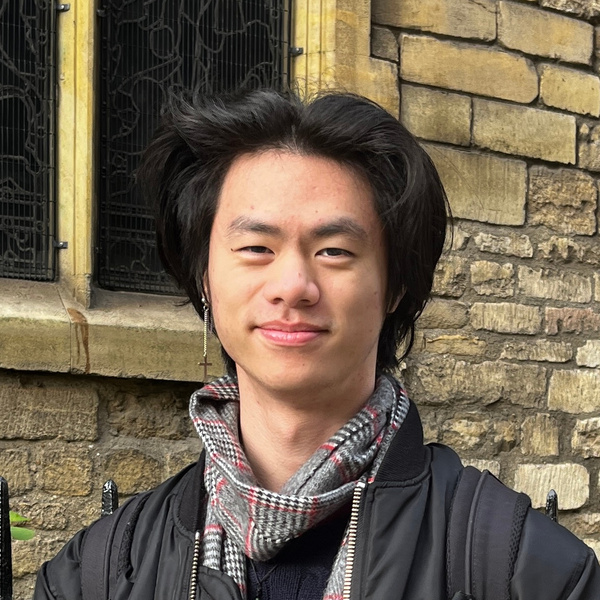
\includegraphics[width=0.08\textheight]{people/ming_yang.jpg}%
        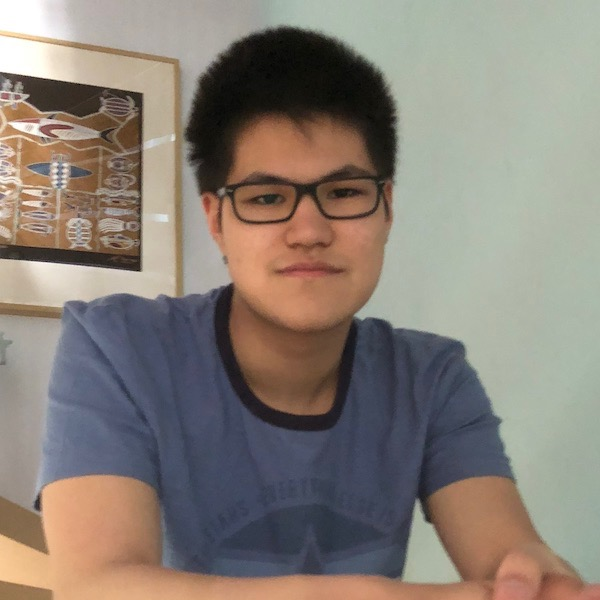
\includegraphics[width=0.08\textheight]{people/namu_kroupa.jpg}%
        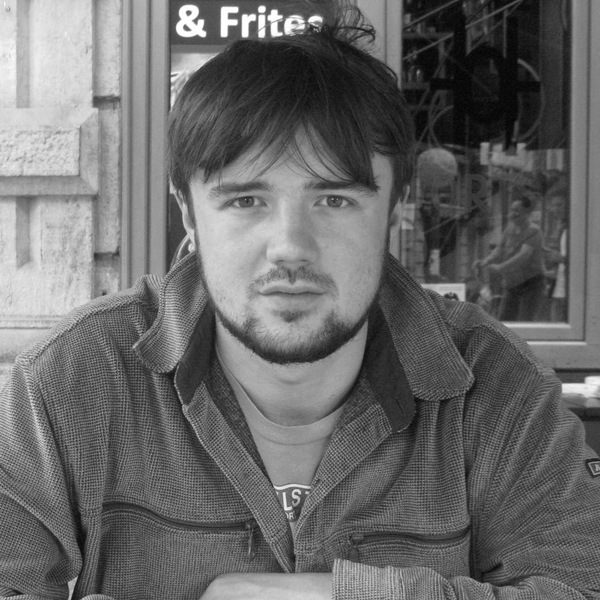
\includegraphics[width=0.08\textheight]{people/sam_leeney.jpg}%
        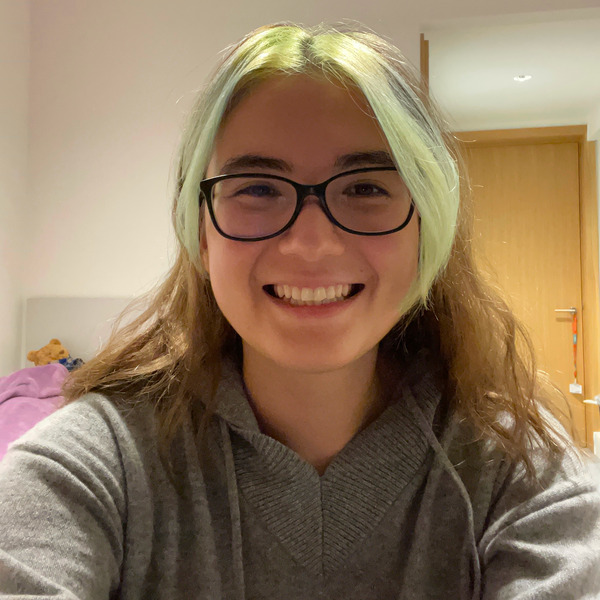
\includegraphics[width=0.08\textheight]{people/sinah_legner.jpg}%
        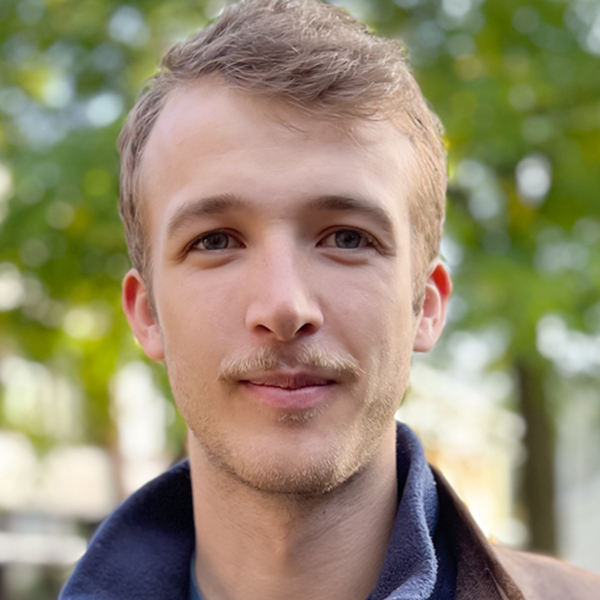
\includegraphics[width=0.08\textheight]{people/toby_lovick.jpg}%
        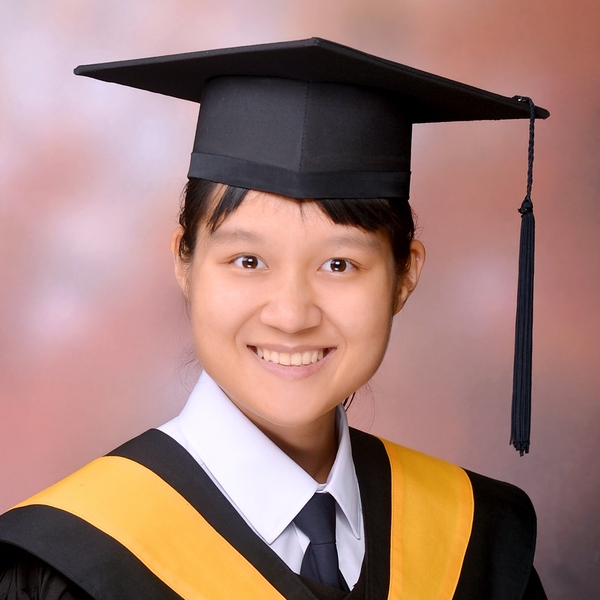
\includegraphics[width=0.08\textheight]{people/wei-ning_deng.jpg}%
        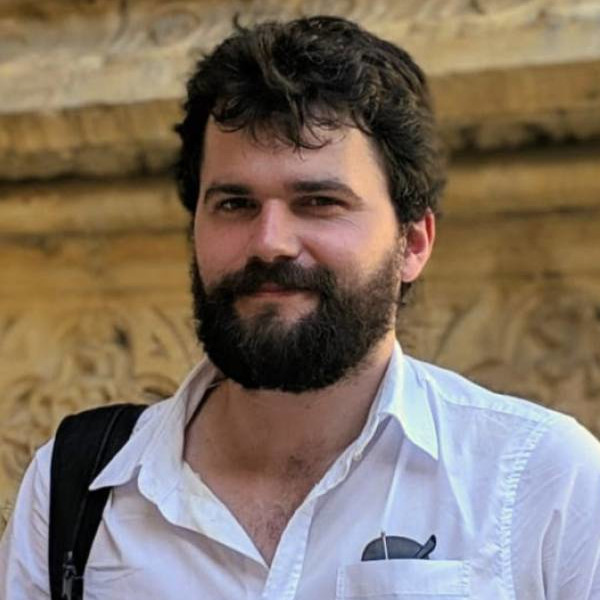
\includegraphics[width=0.08\textheight]{people/will_handley.jpg}%
        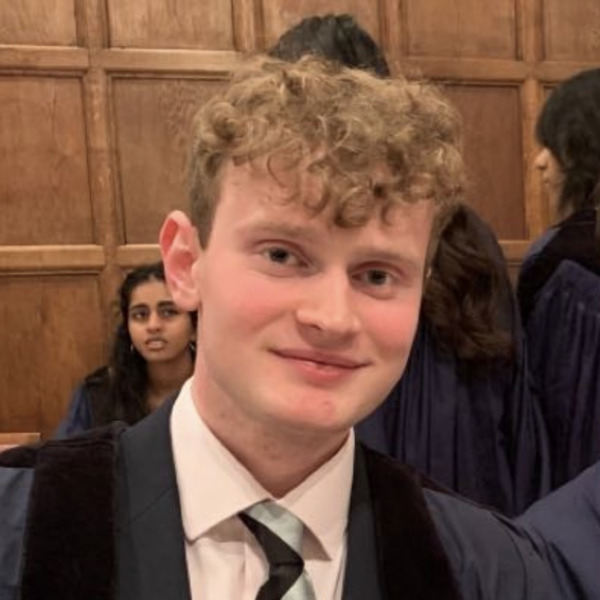
\includegraphics[width=0.08\textheight]{people/will_templeton.jpg}%
    };
\end{frame}

\end{document}
